\documentclass[../main.tex]{subfiles}
\tikzstyle{container} = [draw, rectangle, inner sep=0.3cm]
\begin{document}
The chapter discuss the Software Configuration Manager. This practice is not a development practice, as Scrum, but mainly set guidelines to how the software should be indeed developed. Defining how to treat the artifacts and to keep track of versioning. The chapter introduces then the practice related to continuous integration, delivery and deployment and their relation to SCM. Most of the tools reported are being used during the development of the thesis project 
\section{SCM - Software configuration Management}
Software configuration management is an umbrella of activities that is applied throughout the software development process. The main focus of SCM is related to the changes made during the process. For this reason the main activities of software configuration management are developed to identify changes, control changes, ensure that changes are properly implemented and report changes to to the stakeholders team.\\
SCM is not a methodology such as Scrum, the two coexist in parallel. Changes done working in a Scrum manner are taken care by applying SCM principles.\\
A more theoretical description of SCM comes form \cite{10.1007/978-3-319-32467-8_110}, According to \citet{10.1007/978-3-319-32467-8_110} SCM is defined as the discipline of identifying the configuration of a system at a discrete points in time for purpose of systematically controlling changes to this configuration and maintaining the integrity and traceability of this configuration throughout the system life cycle.
\subsection{SCM Components}
To have a better overview of how the SCM process is structured it´s import at to have an overview of the main tools that are used in the process. The components interacts together to create the system big picture. The main components in Software configuration Managements are:
\begin{itemize}
    \item Software configuration Items; collection of the artifacts created during the software development process. 
    \item Baselines; defines a software configuration in a certain point of times
    \item Repository; container that stores information regarding a system configuration and configuration items. 
    \item Version Control; set of tools and practices to track and manage the development of different Software configuration. 
\end{itemize}
\subsubsection{Software Configuration Items}
Configuration items are a collection of artifacts ranging form software to hardware that need to be managed during the SCM process. In general these items are composed by:
\begin{itemize}
    \item Results of the software development process. 
    \item System specification and system design information
    \item Test data, output of testing phases. 
    \item Documentation
\end{itemize}
The collection of those artifacts is considered as a single entity in the development process and need to be identified uniquely in order to be able to differentiate it from the other configuration items. 
\subsubsection{Baselines}
A baseline is essentially the state of configuration artifacts items that full fill certain criteria at some point in time. A baseline need to withstand both time criteria but also functionality criteria. For software development the functional criteria could be related to passing system test and having no defects with high severity. Having a stable baseline is key in SCM process.\\
All new addiction to the project will be based on a baseline, therefor there is the need for stability to start up on, other than that a baseline is also the starting point to the production baseline, or the project version that is deployed to the customer.\\
In Agile software development a baseline is deployed at the end of a sprint. The project baseline instead can be deployed once every three sprints. 
\subsubsection{Repository}
A repository is simply a structured repository on a server that stores each versioned files separately. The simple definition of repository hide the complexity that the repository structure need to have for complex projects. A project item becomes a Configuration item as soon as it enters a versioned repository. \\
Repository can be organized to differentiate between base and slave directories. Indeed production artifact are stored under strict modification rule, that require all the changes to receive an authorization.  In general repositories are strictly connected with baseline to ensure consistency. 
\subsubsection{Version control}
Version control is essentially the management of changes to a set of configuration items, most commonly source code and documents stored in a repository. Each change creates a new version.\\ 
The main difference between versions and baseline is that each artifacts in a configuration set has its own version, while the group of artifacts with a specific version define a baseline. If only one item in a baseline gets modified, and therefore gets an updated version, then the the configuration set is not in at the baseline level anymore. At the same time in the same baseline can be present artifact whit completely different versions.\\
Some of the main things related to version control are the following:
\begin{itemize}
    \item Check in, define the process of adding or updating an item in a repository. In order to check in in the working directory some type of testing and review is required. For software a requirement could be that the code build and work. 
    \item Check out, process of requesting a version controlled item in order to apply changes on it. After a modification the version control procedure continue with a check-in of the modified item. 
    \item Branching, A branch is a deviation from the main development of a configuration item, and allows for more than one person to work on the same configuration item. A branch can be seen as a image of the repository taken at a certain period of time. On this copy modification can be made and tested. The main goal is the one of keeping a stable main branch (the one on which the baseline stand) and test modification on side branches before merging those modification back on the main branch.
    \item Merging, as noted changes in branches need to be incorporated into the main line for that configuration item. The act of incorporating changes from a branch tin to the main line, or in another branch is called merging. If changes have been made to different parts of an item, e.g., different lines in the source code, the merge is trivial, and can be done automatically by most software. The problem comes if two people have done changes to the same place, then the merge is no longer trivial and has to be handled manually.
\end{itemize}
\section{SCM operations}
SCM activities are organized into four functions:
\begin{itemize}
    \item configuration identification, in this step the configuration items are identified.
    \item configuration control, control the changes to the previously defined configuration items throughout the product life
    \item configuration status accounting, recording and reporting the status of configuration items
    \item configuration audit, verifying the completeness of the items. 
\end{itemize}
The following subsections report the main information's and requirement related to each activities.
\subsubsection{Configuration Identification}
The fist phase in SCM is the identification of Configurations items. In this step the team not only defines which items are worth tracking during the development process, but also identify a structure of such components and a proper naming convention. This make the process of versioning and items accessing easier.\\
Even if the structure can be later adjusted, this steps lay the foundations for the way the project is handled in the future. Therefor an efficient and clear organization is a first step towards SCM success \cite{ieestandard}.
\subsubsection{Configuration control}
Configuration Control is the means to assess and record changes to the functional characteristics of a Configuration Item, revisions to the  Configuration Item definition data and monitoring such changes during preparation, review, approval and implementation. Configuration control activities request, evaluate, approve or disapprove, and implement changes to baselined CIs. Changes can include both error correction and enhancement \cite{ieestandard}.
\subsubsection{Configuration Status Accounting}
Configuration Status Accounting is the means to record and report product configuration evolution history, Change processing and implementation status and Product documentation status and history \cite{ieestandard}.
\subsubsection{Configuration Audit}
Configuration Verification Review and SCM Audit is the means to assess that the final product design is completely documented, the final product design satisfies all performance requirements of the specification(s), the initially produced product meets the design disclosure of its governing documentation, and the Configuration Management assets are sufficient to achieve that goals \cite{ieestandard}.
\section{Software build}
The definition of software build reported by Wikipedia \cite{builddef} refers to build as the process of converting source code files in a standalone software artifacts that can be run on a computer, or the result of doing so. The build build process includes step such as retrieving the correct components, compiling, running scripts that generates source files.\\
\subsection{Relationship between Build process, SCM and Scrum}

\begin{figure}[H]
    \begin{center}
        \begin{tikzpicture}[scale=0.7,transform shape,node distance=4cm,>=latex']
        \node [input3, left of=sum ] (requirements) {$Requirements$};
        \node [sum2, right of=requirements] (sum) {};
        \draw [->] (requirements) -- node [left] {} (sum);
        \node [block, right of=sum] (changes) {$Changes\;Implementation$};
        \draw [->] (sum) -- node {} (changes);
        \node [block, right of=changes] (build) {$Build$};
        \draw [->] (changes) -- node {} (build);
        \node [block, right of=build] (test) {$Test$};
        \draw [->] (build) -- node {} (test);
        \node [block, right of=test] (review) {$Review$};
        \draw [->] (test) -- node {} (review);
        \draw[->] (review)--++(-90:1) coordinate (A)--++(-90:4.5) coordinate (B)-|(sum);
        \node [block, above of=review] (versioning) {$Versioning$};
        \draw [->] (review) -- node [above, pos=0.79] {} (versioning);
        \node [block, above of=versioning] (repository) {$Repository$};
        \draw [<-] (versioning) -- node {} (repository);
        
        \node [block, above of=sum] (branch) {$Branch$};
        \draw [<-] (sum) -- node {} (branch);
        \node [block, above of=branch] (Baseline) {$Baseline$};
        \draw [<-] (branch) -- node {} (Baseline);
        \node [sum2, above of=Baseline] (sum1) {};
        \draw [<-] (Baseline) -- node {} (sum1);
        \draw [->] (repository) |- node {} (sum1);
        
        \node [input2, name=input, left of=sum1] {};
        \draw [draw,->] (input) -- node [above left] {$Other\;changes$} (sum1);
        
        \end{tikzpicture}
    \end{center}
    \caption{Build Approach}\label{figscrum}
\end{figure}
The build process insert itself in the SCM process as the one responsible of modifying the configurations artifacts. Via the build and other auxiliary step the artifact are modified and new are created, requiring therefor all the previously explained SCM operations.  Other than that the build the process is the junction point of SCM with Agile development. 
\begin{figure}
    \centering
    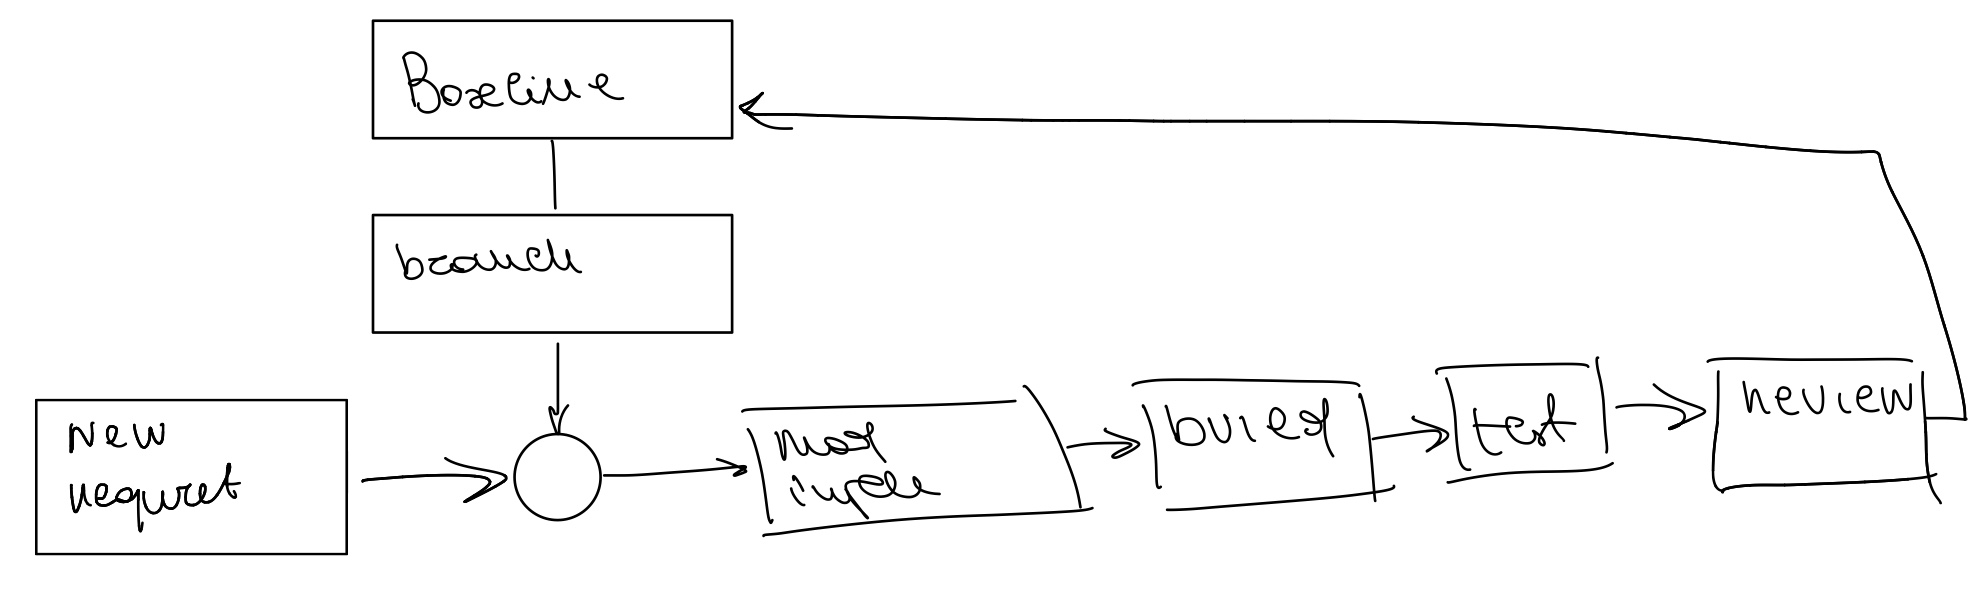
\includegraphics[width=0.8\linewidth]{images_folder/Sdhemabuild.jpeg}
    \caption{Build process}
    \label{fig:build process}
\end{figure}
Modification to the source files mainly comes from a Scrum item. Consider during a Scrum sprint that a changes or a new feature is required for the output artifacts. The modification need to be first implemented in the source code. To do that a branch from the baseline is created. On this branch the modification are implemented by the developer. Once a modification is implemented the build process can start. The artifacts are created. Before those artifacts become part of a configuration items (i.e. before they get proper versioning) they need to be tested. In this case unit test and a review of the output artifacts is implemented. Once all the review process is completed a versioned repository is created. Based on the sum of different mods a new baseline is created. Baselining can be based on number of modification or just on a temporal manner. Baseline have the same time frequency as sprints, this means that once a new sprint start a new baseline is created. There could also be differences between a production baseline, which need to be more stable, and therefor only changes that have passed a lengthy review can be deployed in which a new baseline can be created also once every four or five sprint.\\
Another example, close to the automotive world is the homologation baseline, after a baseline receive the homologation tag, changes allowed are limited or not allowed at all. 
\subsection{Build types}
In general three types of build are part of the environment of SCM. Each type of build has a different scope and also a different frequency at which is run. The main types are:
\begin{itemize}
    \item Private Build, the developer in its own private work space run the build process. As reported next, some build software allow for partial build. The developer can "run" only the part in which the changes have been applied. The developer verify the correctness o of the implemented changes before committing them to the code line where they will be available to the rest of the team. 
    \item Integration build, the integration build is used to incorporate the newly developed changes and verifying that the sum of all the changes output a stable and consistent result. In general this build can therefor be used as a versioned one. Developer are going to use this version to implement further changes. 
    \item Release build, package the software release. The main point is to create the releasable product for the customer. Differently from the integration step, in this step the output product is packed and ready to be deployed to the customer. This may require more steps that are omitted in the integration step. An example can be the creation of documentation or some artifacts useful only for developers. 
\end{itemize}
\subsection{Software build tools}
Software build tools are used to automate the creation of executable application starting from source code. The most basic and most known software build tool is gcc (GNU software build) to create the executable from a generic c file. 
\begin{center}
    \texttt{gcc -o Helloworldexe HelloWorld.c}
\end{center}
In a block scheme manner the task that the gcc build system complete are reported in \ref{Build process overview}:
\tikzstyle{block} = [draw, rectangle, text width=2cm, text centered, minimum height=1.2cm, node distance=3cm]
\begin{figure}[h]
  \centering
\begin{tikzpicture}[scale=0.85,transform shape]
    \node [block, name=text1] {Source code};
    \node [block, right of=text1] (text2) {Compiler};
    \node [block, right of=text2] (text3) {Assembler};
    \node [block, right of=text3] (text4) {Linker};
    \node [block, right of=text4] (text5) {Locator};
    \node [block, right of=text5] (text6) {Executable file};
    \node [container,fit=(text2) (text3) (text4) (text5)] (container) {};

    \draw [->] (text1) -- (text2);
    \draw [->] (text2) -- node {} (text3);
    \draw [->] (text3) -- node {} (text4);
    \draw [->] (text4) -- node {} (text5);
    \draw [->] (text5) -- node {} (text6);
\end{tikzpicture}
  \caption{Build process overview}
\end{figure}
The only taks that are run by gcc is the creation of executable files. More actual software build tools run different tasks such as downloading dependencies, compiling and packing code, running test and deploy artifacts of the build process. The actual usefulness of build tools comes into place in big projects, where it´s hard to keep track of what need to be build, there are complex dependencies and sometimes a single full build can take up also hours. In this case by the use of build tools we can define the dependencies tree and execute tasks sequentially. This mean that via the use of buidl tools the developer can run only the build process from the last modified steps. If a developer implement a mod in the last buidl step then only this is goin to require an update 
\section{Continuous integration}
\cleardoublepage
\end{document}